\begin{frame}
\frametitle{Shopping list: hardware for this course}
  \begin{columns}
    \column{0.85\textwidth}
    \footnotesize
    \begin{itemize}
      \item BeagleBone Black or BeagleBone Black Wireless - Multiple distributors: \\
	    See \url{https://www.beagleboard.org/boards}.
      \item USB Serial Cable - 3.3 V - Female ends (for serial console)
            \footnote{\tiny \url{https://www.olimex.com/Products/Components/Cables/USB-Serial-Cable/USB-SERIAL-F/}}
      \item Nintendo Nunchuk with UEXT connector
            \footnote{\tiny \url{https://www.olimex.com/Products/Modules/Sensors/MOD-WII/MOD-Wii-UEXT-NUNCHUCK/}}
      \item Breadboard jumper wires - Male ends (to connect the Nunchuk)
            \footnote{\tiny \url{https://www.olimex.com/Products/Breadboarding/JUMPER-WIRES/JW-110x10/}}
      \item USB Serial Cable - 3.3 V - Male ends (for serial labs, two if possible)
	    \footnote{\tiny \url{https://www.olimex.com/Products/Components/Cables/USB-Serial-Cable/USB-SERIAL-M/}}
      \item Note that both USB serial cables are the same.\\
            Only the gender of their connector changes.
    \end{itemize}
    \column{0.15\textwidth}
    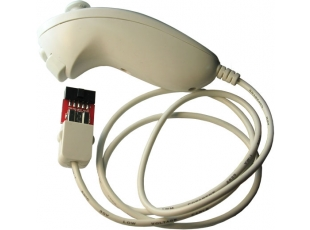
\includegraphics[height=0.25\textheight]{common/nunchuk.jpg} \\
    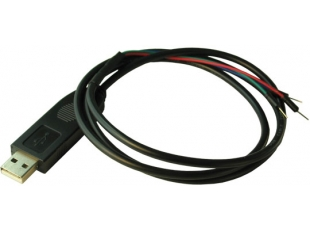
\includegraphics[height=0.20\textheight]{slides/kernel-shopping-list/usb-serial-cable-male.jpg} \\
    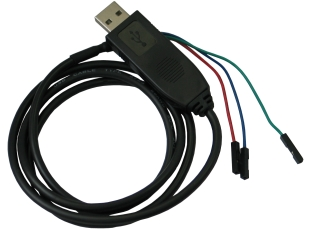
\includegraphics[height=0.20\textheight]{common/usb-serial-cable-female.png} \\
    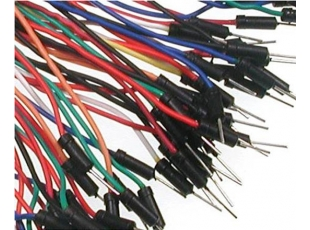
\includegraphics[height=0.15\textheight]{common/jumper-wires.jpg}
  \end{columns}
\end{frame}
